%%%%%%%%%%%%%%%%%%%%%%%%%%%%%%%%%%%%%%%%%%%%%%%%%%%%%%%%%%%%%%%%%%%
%TO AVOID FORMATTING ISSUES, COMPILE THIS ONLY AT WWW.OVERLEAF.COM%
%%%%%%%%%%%%%%%%%%%%%%%%%%%%%%%%%%%%%%%%%%%%%%%%%%%%%%%%%%%%%%%%%%%
%AUTHOR: ABHINAV BAKSHI
%CLASS:  BE C 302
%%%%%%%%%%%%%%%%%%%%%%%%%%%%%%%%%%%%%%%%%%%%%%%%%%%%%%%%%%%%%%%%%%%
\documentclass[a4paper,12pt]{article}
\usepackage{graphicx}
%To use this font, you need XeTex or LuaTex, prefer openleaf
\newenvironment{codefont}{\fontfamily{ccr}\selectfont}{\par}

\title{
	\normalfont \normalsize 
	\textsc{Pimpri Chinchwad College of Engineering \\ 
		Computer Laboratory - IV} \\
	[10pt] 
	\rule{\linewidth}{0.5pt} \\[6pt] 
	\huge Assignment No - B1 \\
	\rule{\linewidth}{2pt}  \\[10pt]
}
\author{}
\date{\normalsize}


\begin{document}
\maketitle

%%%%%%%%%%%%%%%%%%%%%%%
% FOR A NUMBERED LIST
% \begin{enumerate}
% \item Your_Item
% \end{enumerate}
%%%%%%%%%%%%%%%%%%%%%%%
% FOR A BULLETED LIST
% \begin{itemize}
% \item Your_Item
% \end{itemize}
%%%%%%%%%%%%%%%%%%%%%%%
% TO IMPORT AN IMAGE
% \includegraphics[width=\textwidth]{name_of_file}
% \textwidth makes the picture the width of the paragraphs
%%%%%%%%%%%%%%%%%%%%%%%%%%%%%%
% TO CREATE A FIGURE WITH A NUMBER AND CAPTION
% \begin{figure}
% \includegraphics[width=\textwidth]{image}
% \caption{Your Caption Goes Here}
% \label{your_label}
% \end{figure}
% REFER TO YOUR FIGURE LATER WITH
% \ref{your_label}
% LABELS NEED TO BE ONE WORD
%%%%%%%%%%%%%%%%%%%%%%%%%%%%%
% TO ADD CODE
% \begin{codefont}
% Some code in "courier" font
%\end{codefont}
%%%%%%%%%%%%%%%%%%%%%%%%%%%%%
\section{Aim}
	\paragraph{} 8-Queens Matrix is Stored using JSON/XML having first Queen placed, use back-tracking to place
	remaining Queens to generate final 8-queen’s Matrix using Python. Create a backtracking scenario and
	use HPC architecture (Preferably BBB) for computation of next placement of a queen.
	
\section{Objective}
	\begin{itemize}
		\item To study 8 Queens problem, and implement it using Python 
	\end{itemize}
	
\section{Software Requirements}
	\begin{itemize}
		\item	Linux
		\item   Python
	\end{itemize}
	
\section{Mathematical Model}
	\begin{flushleft}
		\textbf{Input : }  Size of Board and Initial state of queen.\\
		\textbf{Output : } 8 queen placed in 8*8 matrix in such a way that they do not attack each other.\\
		\textbf{Formula:}
	\end{flushleft}•
	int PlaceQueen(int board[8], int row)  \\
	If (Can place queen on ith column)  \\
	PlaceQueen(newboard, 0)\\
	Else  \\
	PlaceQueen(oldboard,oldplace+1) \\
	End
	
\section{Theory}

\subsection{8-queen}
	The 8 queen problem is a case of more general set of problems namely “n queen problem”. The basic idea: How to place n queen on n by n board, so that they don’t attack each other.
	
	As we can expect the complexity of solving the problem increases with n. We will briefly introduce solution by backtracking.  First let’s explain what is backtracking? The boar should be regarded as a set of constraints and the solution is simply satisfying all constraints. 
	
	For example: Q1 attacks some positions, therefore Q2 has to comply with these constraints and take place, not directly attacked by Q1. Placing Q3 is harder, since we have to satisfy constraints of Q1 and Q2. 
	
	Going the same way we may reach point, where the constraints make the placement of the next queen impossible. Therefore we need to relax the constraints and find new solution. To do this we are going backwards and finding new admissible solution. To keep everything in order we keep the simple rule: last placed, first displaced. 
	
	In other words if we place successfully queen on the ith column but cannot find solution for$ (i+1)th$ queen, then going backwards we will try to find other admissible solution for the ith queen first. This process is called backtrack  .\\
		
\subsection{Beaglebone Black}
	\textbf{BeagleBone Black Overview:}\\ 
	The BeagleBone Black is the latest addition to the BeagleBoard.org family and like its predecessors, is designed to address the Open Source Community, early adopters, and anyone interested in a low cost ARM Cortex-A8 based processor. It has been equipped with a minimum set of features to allow the user to experience the power of the processor and is not intended as a full development platform as many of the features and interfaces supplied by the processor are not accessible from the Beagle Bone Black via on board support of some interfaces. It is not a complete product designed to do any particular function. It is a foundation for experimentation and learning how to program the processor and to access the peripherals by the creation of your own software and hardware. It also offers access to many of the interfaces and allows for the use of add-on boards called capes, to add many different combinations of features. A user may also develop their own board or add their own circuitry.
	
	\textbf{Board Component Locations:}\\ 
	This section describes the key components on the board. It provides information on their location and function. Familiarize yourself with the various components on the board. 
	\begin{itemize}
	\item Connectors, LEDs, and Switches 
	\item DC Power is the main DC input that accepts 5V power. 
	\item Power Button alerts the processor to initiate the power down sequence.  
	\item 10/100 Ethernet is the connection to the LAN. 
	\item Serial Debug is the serial debug port. 
	\item USB Client is a mini USB connection to a PC that can also power the board. 
	\item BOOT switch can be used to force a boot from the SD card. 
	\item There are four blue LEDS that can be used by the user. 
	\item Reset Button allows the user to reset the processor. 
	\item uSD slot is where a uSD card can be installed. 
	\item microHDMI connector is where the display is connected to. 
	\item USB Host can be connected different USB interfaces such asWi-Fi, BT,Keyboard, etc  	
	\end{itemize}
	
	\textbf{Features of Beaglebone Black}\\
	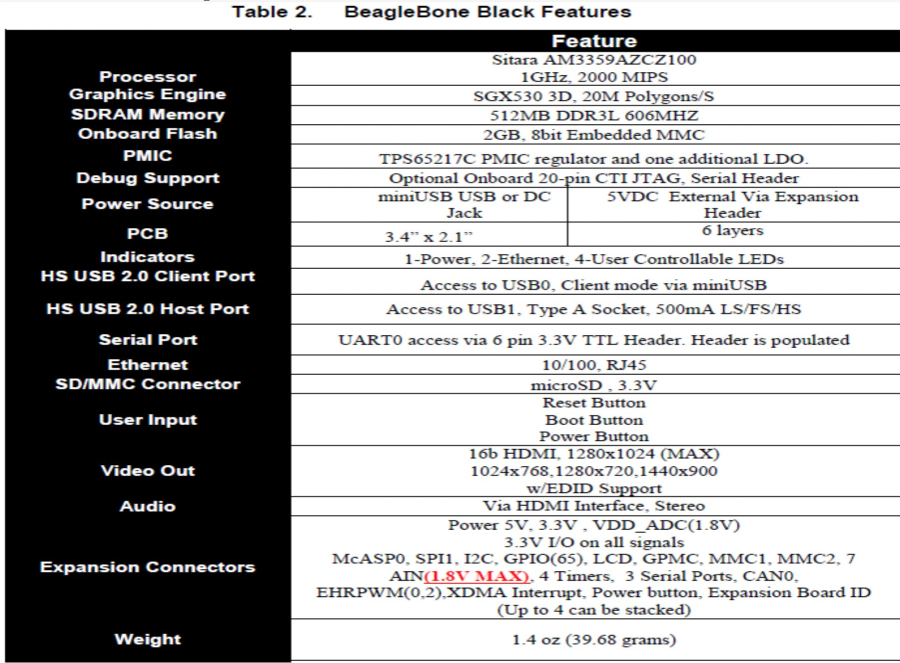
\includegraphics[width=\textwidth]{features_bbb.png}
	
	\textbf{Key Components}
	\begin{itemize}
		\item Sitara AM3359AZCZ100 is the processor for the board. 
		\item Micron 512MB DDR3L is the Dual Data Rate RAM memory. 
		\item TPS65217C PMIC provides the power rails to the various components on the board. 
		\item SMSC Ethernet PHY is the physical interface to the network. 
		\item Micron eMMC is an onboard MMC chip that holds up to 2GB of data. 
		\item HDMI Framer provides control for an HDMI or DVI-D display with an adapter. 
	\end{itemize}
	\vspace{30px}
	
	
	\textbf{Connectivity}
	\begin{itemize}
		\item Connect the small connector on the USB cable to the board as shown in Figure 1. The connector is on the bottom side of the board. 
		\item Connect the large connector of the USB cable to your PC or laptop USB port. 
		\item The board will power on and the power LED will be on as shown in Figure 2 below. 
	\end{itemize}
	
		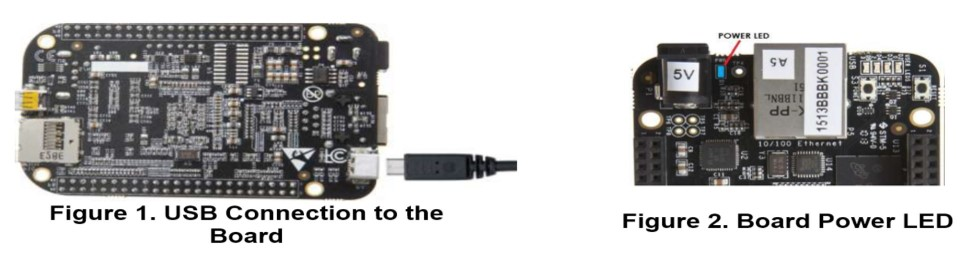
\includegraphics[width=\textwidth]{bbb_01}
	
	\begin{itemize}
		\item Apply Power: 
		The final step is to plug in the DC power supply to the DC power jack as shown in Figure4 below. 
		
		\item Booting the Board: 
		As soon as the power is applied to the board, it will start the booting up process. When the board starts to boot the LEDs will come on in sequence as shown in Figure 5 below. It will take a few seconds for the status LEDs to come on, so be patient. The LEDs will be flashing in an erratic manner as it boots the Linux kernel. 
	\end{itemize}
	
	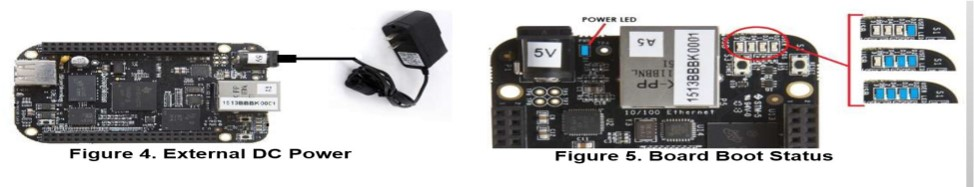
\includegraphics[width=\textwidth]{bbb_02}
	
\subsection{Steps to run program in Beaglebone Black}
	1.	In red hat terminal we need to type following command for accessing the beagle bone terminal. 
	ssh 192.168.7.2 \\
	2.	Open another redhat terminal for copying the python program from redhat to beagle bone by using command: 
	scp filename.py root@192.168.7.2: \\
	3.	Now open beagle bone terminal to check whether program is copied or not by using command ls. \\
	4.	To run the program write following command in beagle bone terminal. 
	python filename.py \\
	
	 
			
		
\section{Testing}
	\subsection{Black Box Testing}
	Black-box testing is a method of software testing that examines the\\ function- ability of an application without peering into its internal structures or workings.\\
	This method of test can be applied to virtually every level of\\ software testing:unit, integration, system and acceptance\\
	Typical Input Data:  Position of first queen\\
	Expected Output: Possible positions of remaining 7 queens to satisfy the 8 – Queen Problem\\
	
	\noindent Example:\\
	Input: \\
	$$X = 4 , Y = 4$$
	
	Output:\\
	$[2, 0, 6, 4, 7, 1, 3, 5]$\\
	$[2, 5, 1, 4, 7, 0, 6, 3]$\\
	$[3, 1, 6, 4, 0, 7, 5, 2]$\\
	$[3, 1, 7, 4, 6, 0, 2, 5]$\\
	$[3, 5, 0, 4, 1, 7, 2, 6]$\\
	$[3, 7, 0, 4, 6, 1, 5, 2]$\\
	$[5, 3, 0, 4, 7, 1, 6, 2]$\\
	$[6, 3, 1, 4, 7, 0, 2, 5]$\\
	8\\
	
	\subsection{White Box Testing}
	White-box testing (also known as clear box testing, glass box testing, transparent box testing, and structural testing) is a method of testing software that tests internal structures or workings of an application, as opposed to its functionality(i.e. black-box testing). While developing 
	test cases for white box testing it is understood that complete testing 
	is impossible. In White Box testing we checkup to which extent the code 
	is being executed, i.e. Covered. There are different kinds of coverage like, statement coverage, path coverage, etc. We will use one of the most popular technique i.e. Statement coverage. Statement coverage is a white box testing technique, which involves the execution of all the statements at least once in the source code. It is a metric, which is used to calculate and measure the number of statements in the source code which have been executed. For this, we will use Flow Graphs. Flow graphs are, Syntactic abstraction of source code Resembling to classical flow charts Forms the basis for white box test case generation principles.Conventions of flow graph notation, \\
	Sample Input: For integer array int A[] = 1,2,3,4,5,6,7,8,9,10; Function 
	is passed\\
	following arguments: Binary Search(A, 1, 10, 7);\\
	Output obtained: Entered second Entered third Entered first 6\\
	The underlined nodes are the ones being tested. The above output shows
	that every test region is covered for given input.\\
	
	\begin{figure}[h!]
		\centering
		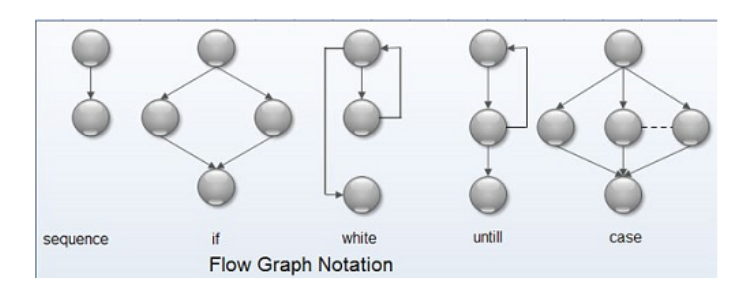
\includegraphics[scale=0.5]{pqr.png}
		\end{figure}
		
		\begin{figure}[h!]
			\centering
			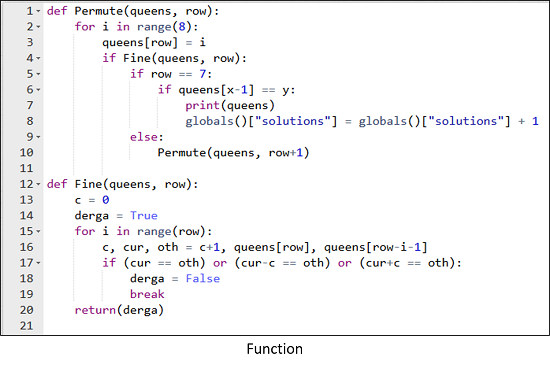
\includegraphics{quee.png}
			\end{figure}	
			
			\begin{figure}[h!]
				\centering
				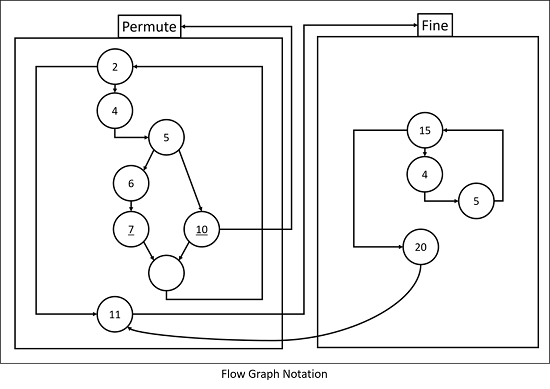
\includegraphics{qu.png}
				\end{figure}
				
				\noindent
				Sample Input:\\
				Given coordinates (X,Y) = 4,4\\
				\noindent
				Output obtained:\\
				
				$Valid Case   : [0, 4, 7, 5, 2, 6, 1, 3]$\\
				$Valid Case   : [0, 5, 7, 2, 6, 3, 1, 4]$\\
				$Valid Case   : [0, 6, 3, 5, 7, 1, 4, 2]$\\
				$Valid Case   : [0, 6, 4, 7, 1, 3, 5, 2]$\\
				$Valid Case   : [1, 3, 5, 7, 2, 0, 6, 4]$\\
				$Valid Case   : [1, 4, 6, 0, 2, 7, 5, 3]$\\
				$Valid Case   : [1, 4, 6, 3, 0, 7, 5, 2]$\\
				$Valid Case   : [1, 5, 0, 6, 3, 7, 2, 4]$\\
				$Valid Case   : [1, 5, 7, 2, 0, 3, 6, 4]$\\
				$Valid Case   : [1, 6, 2, 5, 7, 4, 0, 3]$\\
				$Valid Case   : [1, 6, 4, 7, 0, 3, 5, 2]$\\
				$Valid Case   : [1, 7, 5, 0, 2, 4, 6, 3]$\\
				$Solution Case: [2, 0, 6, 4, 7, 1, 3, 5]$\\
				$Valid Case   : [2, 0, 6, 4, 7, 1, 3, 5]$\\
				$Valid Case   : [2, 4, 1, 7, 0, 6, 3, 5]$\\
				$Valid Case   : [2, 4, 1, 7, 5, 3, 6, 0]$\\
				$Valid Case   : [2, 4, 6, 0, 3, 1, 7, 5]$\\
				$Valid Case   : [2, 4, 7, 3, 0, 6, 1, 5]$\\
				$Solution Case: [2, 5, 1, 4, 7, 0, 6, 3]$\\
				$Valid Case   : [2, 5, 1, 4, 7, 0, 6, 3]$\\
				$Valid Case   : [2, 5, 1, 6, 0, 3, 7, 4]$\\
				$Valid Case   : [2, 5, 1, 6, 4, 0, 7, 3]$\\
				$Valid Case   : [2, 5, 3, 0, 7, 4, 6, 1]$\\
				$Valid Case   : [2, 5, 3, 1, 7, 4, 6, 0]$\\
				$Valid Case   : [2, 5, 7, 0, 3, 6, 4, 1]$\\
				$Valid Case   : [2, 5, 7, 0, 4, 6, 1, 3]$\\
				$Valid Case   : [2, 5, 7, 1, 3, 0, 6, 4]$\\
				$Valid Case   : [2, 6, 1, 7, 4, 0, 3, 5]$\\
				$Valid Case   : [2, 6, 1, 7, 5, 3, 0, 4]$\\
				$Valid Case   : [2, 7, 3, 6, 0, 5, 1, 4]$\\
				$Valid Case   : [3, 0, 4, 7, 1, 6, 2, 5]$\\
				$Valid Case   : [3, 0, 4, 7, 5, 2, 6, 1]$\\
				$Valid Case   : [3, 1, 4, 7, 5, 0, 2, 6]$\\
				$Valid Case   : [3, 1, 6, 2, 5, 7, 0, 4]$\\
				$Valid Case   : [3, 1, 6, 2, 5, 7, 4, 0]$\\
				$Solution Case: [3, 1, 6, 4, 0, 7, 5, 2]$\\
				$Valid Case   : [3, 1, 6, 4, 0, 7, 5, 2]$\\
				$Solution Case: [3, 1, 7, 4, 6, 0, 2, 5]$\\
				$Valid Case   : [3, 1, 7, 4, 6, 0, 2, 5]$\\
				$Valid Case   : [3, 1, 7, 5, 0, 2, 4, 6]$\\
				$Solution Case: [3, 5, 0, 4, 1, 7, 2, 6]$\\
				$Valid Case   : [3, 5, 0, 4, 1, 7, 2, 6]$\\
				$Valid Case   : [3, 5, 7, 1, 6, 0, 2, 4]$\\
				$Valid Case   : [3, 5, 7, 2, 0, 6, 4, 1]$\\
				$Valid Case   : [3, 6, 0, 7, 4, 1, 5, 2]$\\
				$Valid Case   : [3, 6, 2, 7, 1, 4, 0, 5]$\\
				$Valid Case   : [3, 6, 4, 1, 5, 0, 2, 7]$\\
				$Valid Case   : [3, 6, 4, 2, 0, 5, 7, 1]$\\
				$Valid Case   : [3, 7, 0, 2, 5, 1, 6, 4]$\\
				$Solution Case: [3, 7, 0, 4, 6, 1, 5, 2]$\\
				$Valid Case   : [3, 7, 0, 4, 6, 1, 5, 2]$\\
				$Valid Case   : [3, 7, 4, 2, 0, 6, 1, 5]$\\
				$Valid Case   : [4, 0, 3, 5, 7, 1, 6, 2]$\\
				$Valid Case   : [4, 0, 7, 3, 1, 6, 2, 5]$\\
				$Valid Case   : [4, 0, 7, 5, 2, 6, 1, 3]$\\
				$Valid Case   : [4, 1, 3, 5, 7, 2, 0, 6]$\\
				$Valid Case   : [4, 1, 3, 6, 2, 7, 5, 0]$\\
				$Valid Case   : [4, 1, 5, 0, 6, 3, 7, 2]$\\
				$Valid Case   : [4, 1, 7, 0, 3, 6, 2, 5]$\\
				$Valid Case   : [4, 2, 0, 5, 7, 1, 3, 6]$\\
				$Valid Case   : [4, 2, 0, 6, 1, 7, 5, 3]$\\
				$Valid Case   : [4, 2, 7, 3, 6, 0, 5, 1]$\\
				$Valid Case   : [4, 6, 0, 2, 7, 5, 3, 1]$\\
				$Valid Case   : [4, 6, 0, 3, 1, 7, 5, 2]$\\
				$Valid Case   : [4, 6, 1, 3, 7, 0, 2, 5]$\\
				$Valid Case   : [4, 6, 1, 5, 2, 0, 3, 7]$\\
				$Valid Case   : [4, 6, 1, 5, 2, 0, 7, 3]$\\
				$Valid Case   : [4, 6, 3, 0, 2, 7, 5, 1]$\\
				$Valid Case   : [4, 7, 3, 0, 2, 5, 1, 6]$\\
				$Valid Case   : [4, 7, 3, 0, 6, 1, 5, 2]$\\
				$Valid Case   : [5, 0, 4, 1, 7, 2, 6, 3]$\\
				$Valid Case   : [5, 1, 6, 0, 2, 4, 7, 3]$\\
				$Valid Case   : [5, 1, 6, 0, 3, 7, 4, 2]$\\
				$Valid Case   : [5, 2, 0, 6, 4, 7, 1, 3]$\\
				$Valid Case   : [5, 2, 0, 7, 3, 1, 6, 4]$\\
				$Valid Case   : [5, 2, 0, 7, 4, 1, 3, 6]$\\
				$Valid Case   : [5, 2, 4, 6, 0, 3, 1, 7]$\\
				$Valid Case   : [5, 2, 4, 7, 0, 3, 1, 6]$\\
				$Valid Case   : [5, 2, 6, 1, 3, 7, 0, 4]$\\
				$Valid Case   : [5, 2, 6, 1, 7, 4, 0, 3]$\\
				$Valid Case   : [5, 2, 6, 3, 0, 7, 1, 4]$\\
				$Solution Case: [5, 3, 0, 4, 7, 1, 6, 2]$\\
				$Valid Case   : [5, 3, 0, 4, 7, 1, 6, 2]$\\
				$Valid Case   : [5, 3, 1, 7, 4, 6, 0, 2]$\\
				$Valid Case   : [5, 3, 6, 0, 2, 4, 1, 7]$\\
				$Valid Case   : [5, 3, 6, 0, 7, 1, 4, 2]$\\
				$Valid Case   : [5, 7, 1, 3, 0, 6, 4, 2]$\\
				$Valid Case   : [6, 0, 2, 7, 5, 3, 1, 4]$\\
				$Valid Case   : [6, 1, 3, 0, 7, 4, 2, 5]$\\
				$Valid Case   : [6, 1, 5, 2, 0, 3, 7, 4]$\\
				$Valid Case   : [6, 2, 0, 5, 7, 4, 1, 3]$\\
				$Valid Case   : [6, 2, 7, 1, 4, 0, 5, 3]$\\
				$Solution Case: [6, 3, 1, 4, 7, 0, 2, 5]$\\
				$Valid Case   : [6, 3, 1, 4, 7, 0, 2, 5]$\\
				$Valid Case   : [6, 3, 1, 7, 5, 0, 2, 4]$\\
				$Valid Case   : [6, 4, 2, 0, 5, 7, 1, 3]$\\
				$Valid Case   : [7, 1, 3, 0, 6, 4, 2, 5]$\\
				$Valid Case   : [7, 1, 4, 2, 0, 6, 3, 5]$\\
				$Valid Case   : [7, 2, 0, 5, 1, 4, 6, 3]$\\
				$Valid Case   : [7, 3, 0, 2, 5, 1, 6, 4]$\\
				8
				
				\subsection{Positive Negative Testing}
				
				\textbf{Positive Testing :}\\
				If proper position is entered then all solutions are found.\\
				\textbf{ Negative Testing :}\\
				if uknown position is entered the program must fail to produce outputs
				
				
				\subsection{Advanced Testing Technique}
				Google Testing Framework can be used in future for testing the code

\section{Algorithm}
        \#move right(column increment)\\
        for col in range(1, size + 1):\\
	        \#skip the row in which queen was placed initially\\
	        if row == x and col == y:\\
		        placequeen(row + 1)\\
	        if not danger(row, col):\\
		        board.append((row, col))\\
		        \#move down(row increment)\\
		        placequeen(row + 1)\\
		        board.remove((row,col))\\


\section{Conclusion}
	\paragraph{} We have studied 8 - Queens problem  and have successfully implemented it in python.
	
\vspace{20px}
\begin{center}
	\begin{tabular}
		{|c|c|c|c|}\hline
		{\bf Roll No.}		&{\bf Name of Student}		&{\bf Date of Performance}  				&{\bf Date of Submission}  \\ \hline
		{302}	&	{Abhinav Bakshi}& {20/1/16}		&  {3/2/16}\\ \hline
	\end{tabular}\\ 
\end{center}

\section{Plagarism Report}
		\begin{figure}[h!]
			\centering
			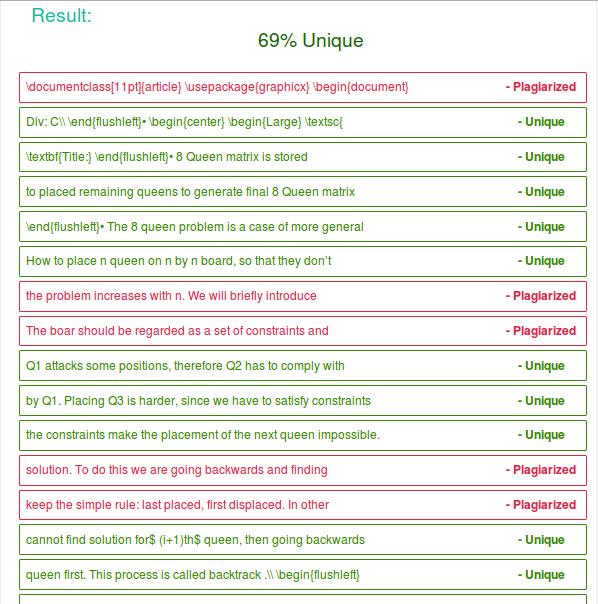
\includegraphics{8Queen_Plag.png}
			\caption{Plagarism Checker: www.smallseotools.com/plagarism-checker}
		\end{figure}
\end{document}
 

 
